\documentclass[11pt,oneside]{article}
\usepackage[T1]{fontenc}
\usepackage[utf8]{inputenc}
% \usepackage{lmodern}
%\usepackage[adobe-utopia,uppercase=upright,greeklowercase=upright]{mathdesign}
\usepackage[adobe-utopia]{mathdesign}
%\usepackage{minionpro}
% \usepackage{pifont}
% \usepackage{amssymb}
\usepackage{amsmath}
\usepackage[francais]{babel}
% \usepackage[francais]{varioref}
\usepackage[dvips]{graphicx}

\usepackage{framed}
\usepackage[normalem]{ulem}
\usepackage{fancyhdr}
\usepackage{titlesec}
\usepackage{vmargin}
\usepackage{longtable}

\usepackage{ifthen}


%\usepackage{epsfig}
\usepackage{subfig}

\usepackage{multirow}
\usepackage{multicol} % Portions de texte en colonnes
\usepackage{flafter}%floatants après la référence



\usepackage{color}
\usepackage{colortbl}


\definecolor{gris25}{gray}{0.75}
\definecolor{bleu}{RGB}{18,33,98}
\definecolor{bleuf}{RGB}{42,94,171}
\definecolor{bleuc}{RGB}{231,239,247}
\definecolor{rougef}{RGB}{185,18,27}
\definecolor{rougec}{RGB}{255,230,231}
\definecolor{vertf}{RGB}{103,126,82}
\definecolor{vertc}{RGB}{220,255,191}
\definecolor{violetf}{RGB}{112,48,160}
\definecolor{violetc}{RGB}{230,224,236}

\newenvironment{sci}[1][\hsize]%
{%
    \def\FrameCommand%
    {%
%\rotatebox{90}{\textit{\textsf{Scilab}}
\includegraphics[height=.8cm]{png/logo_scilab}} 
\rotatebox{90}{
\includegraphics[height=.6cm]{png/logo_scilab}} 
        {\color{violetf}\vrule width 3pt}%
        \hspace{0pt}%must no space.
        \fboxsep=\FrameSep\colorbox{violetc}%
    }%
    \MakeFramed{\hsize #1 \advance\hsize-\width\FrameRestore}%
}%
{\endMakeFramed}%

\newenvironment{pseudo}[1][\hsize]%
{%
    \def\FrameCommand%
    {%
\rotatebox{90}{\textit{\textsf{Pseudo Code}}} 
        {\color{violetf}\vrule width 3pt}%
        \hspace{0pt}%must no space.
        \fboxsep=\FrameSep\colorbox{violetc}%
    }%
    \MakeFramed{\hsize #1 \advance\hsize-\width\FrameRestore}%
}%
{\endMakeFramed}%

\newenvironment{py}[1][\hsize]%
{%
    \def\FrameCommand%
    {%
%\rotatebox{90}{\textit{\textsf{Python}}} 
\rotatebox{90}{
\includegraphics[height=.6cm]{png/logo_python}} 
        {\color{violetf}\vrule width 3pt}%
        \hspace{0pt}%must no space.
        \fboxsep=\FrameSep\colorbox{violetc}%
    }%
    \MakeFramed{\hsize #1 \advance\hsize-\width\FrameRestore}%
}%
{\endMakeFramed}%


\newenvironment{corrige}[1][\hsize]%
{%
    \def\FrameCommand
    {%
\rotatebox{90}{\textit{\textsf{Correction}}} 
        {\color{violetf}\vrule width 3pt}%
        \hspace{0pt}%must no space.
        \fboxsep=\FrameSep\colorbox{violetc}%
    }%
    \MakeFramed{\hsize#1\advance\hsize-\width\FrameRestore}%
}%
{\endMakeFramed}%



\newenvironment{rem}[1][\hsize]%
{%
    \def\FrameCommand
    {%
\rotatebox{90}{\textit{\textsf{Remarque}}} 
        {\color{bleuf}\vrule width 3pt}%
        \hspace{0pt}%must no space.
        \fboxsep=\FrameSep\colorbox{bleuc}%
    }%
    \MakeFramed{\hsize#1\advance\hsize-\width\FrameRestore}%
}%
{\endMakeFramed}%


\newenvironment{savoir}[1][\hsize]%
{%
    \def\FrameCommand
    {%
\rotatebox{90}{\textit{\textsf{Savoir}}} 
        {\color{bleuf}\vrule width 3pt}%
        \hspace{0pt}%must no space.
        \fboxsep=\FrameSep\colorbox{bleuc}%
    }%
    \MakeFramed{\hsize#1\advance\hsize-\width\FrameRestore}%
}%
{\endMakeFramed}%

\newenvironment{prob}[1][\hsize]%
{%
    \def\FrameCommand%
    {%
\rotatebox{90}{\textit{\textsf{ Problématique}}} 
        {\color{rougef}\vrule width 3pt}%
        \hspace{0pt}%must no space.
        \fboxsep=\FrameSep\colorbox{rougec}%
    }%
    \MakeFramed{\hsize#1\advance\hsize-\width\FrameRestore}%
}%
{\endMakeFramed}%

\newenvironment{obj}[1][\hsize]%
{%
    \def\FrameCommand%
    {%
\rotatebox{90}{\textit{\textsf{Objectifs}}} 
        {\color{rougef}\vrule width 3pt}%
        \hspace{0pt}%must no space.
        \fboxsep=\FrameSep\colorbox{rougec}%
    }%
    \MakeFramed{\hsize#1\advance\hsize-\width\FrameRestore}%
}%
{\endMakeFramed}%

\newenvironment{defi}[1][\hsize]%
{%
    \def\FrameCommand%
    {%
\rotatebox{90}{\textit{\textsf{Définition\\}}} 
        {\color{bleuf}\vrule width 3pt}%
        \hspace{0pt}%must no space.
        \fboxsep=\FrameSep\colorbox{bleuc}%
    }%
    \MakeFramed{\hsize#1\advance\hsize-\width\FrameRestore}%
}%
{\endMakeFramed}%


\newenvironment{demo}[1][\hsize]%
{%
    \def\FrameCommand%
    {%
\rotatebox{90}{\textit{\textsf{Démonstration\\}}} 
        {\color{bleuf}\vrule width 3pt}%
        \hspace{0pt}%must no space.
        \fboxsep=\FrameSep\colorbox{bleuc}%
    }%
    \MakeFramed{\hsize#1\advance\hsize-\width\FrameRestore}%
}%
{\endMakeFramed}%


\newenvironment{hypo}[1][\hsize]%
{%
    \def\FrameCommand%
    {%
\rotatebox{90}{\textit{\textsf{Hypothèse\\}}} 
        {\color{bleuf}\vrule width 3pt}%
        \hspace{0pt}%must no space.
        \fboxsep=\FrameSep\colorbox{bleuc}%
    }%
    \MakeFramed{\hsize#1\advance\hsize-\width\FrameRestore}%
}%
{\endMakeFramed}%


\newenvironment{prop}[1][\hsize]%
{%
    \def\FrameCommand%
    {%
\rotatebox{90}{\textit{\textsf{Propriété\\}}} 
        {\color{bleuf}\vrule width 3pt}%
        \hspace{0pt}%must no space.
        \fboxsep=\FrameSep\colorbox{bleuc}%
    }%
    \MakeFramed{\hsize#1\advance\hsize-\width\FrameRestore}%
}%
{\endMakeFramed}%

\newenvironment{props}[1][\hsize]%
{%
    \def\FrameCommand%
    {%
\rotatebox{90}{\textit{\textsf{Propriétés\\}}} 
        {\color{bleuf}\vrule width 3pt}%
        \hspace{0pt}%must no space.
        \fboxsep=\FrameSep\colorbox{bleuc}%
    }%
    \MakeFramed{\hsize#1\advance\hsize-\width\FrameRestore}%
}%
{\endMakeFramed}%

\newenvironment{exemple}[1][\hsize]%
{%
    \def\FrameCommand%
    {%
\rotatebox{90}{\textit{\textsf{Exemple\\}}} 
        {\color{vertf}\vrule width 3pt}%
        \hspace{0pt}%must no space.
        \fboxsep=\FrameSep\colorbox{vertc}%
    }%
    \MakeFramed{\hsize#1\advance\hsize-\width\FrameRestore}%
}%
{\endMakeFramed}%

\newenvironment{resultat}[1][\hsize]%
{%
    \def\FrameCommand%
    {%
\rotatebox{90}{\textit{\textsf{Résultat\\}}} 
        {\color{rougef}\vrule width 3pt}%
        \hspace{0pt}%must no space.
        \fboxsep=\FrameSep\colorbox{rougec}%
    }%
    \MakeFramed{\hsize#1\advance\hsize-\width\FrameRestore}%
}%
{\endMakeFramed}%

\newenvironment{methode}[1][\hsize]%
{%
    \def\FrameCommand%
    {%
\rotatebox{90}{\textit{\textsf{Méthode\\}}} 
        {\color{rougef}\vrule width 3pt}%
        \hspace{0pt}%must no space.
        \fboxsep=\FrameSep\colorbox{rougec}%
    }%
    \MakeFramed{\hsize#1\advance\hsize-\width\FrameRestore}%
}%
{\endMakeFramed}%

\newenvironment{theo}[1][\hsize]%
{%
    \def\FrameCommand%
    {%
\rotatebox{90}{\textit{\textsf{Théorème\\}}} 
        {\color{rougef}\vrule width 3pt}%
        \hspace{0pt}%must no space.
        \fboxsep=\FrameSep\colorbox{rougec}%
    }%
    \MakeFramed{\hsize#1\advance\hsize-\width\FrameRestore}%
}%
{\endMakeFramed}%

\newenvironment{warn}[1][\hsize]%
{%
    \def\FrameCommand%
    {%
\rotatebox{90}{\textit{\textsf{Attention\\}}} 
        {\color{rougef}\vrule width 3pt}%
        \hspace{0pt}%must no space.
        \fboxsep=\FrameSep\colorbox{rougec}%
    }%
    \MakeFramed{\hsize#1\advance\hsize-\width\FrameRestore}%
}%
{\endMakeFramed}%

% \usepackage{pstricks}
%\usepackage{minitoc}
% \setcounter{minitocdepth}{4}

\setcounter{tocdepth}{2}

% \mtcselectlanguage{french} 

%\usepackage{draftcopy}% "Brouillon"
% \usepackage{floatflt}
\usepackage{psfrag}
%\usepackage{listings} % Permet d'insérer du code de programmation
\renewcommand{\baselinestretch}{1.2}

% Changer la numérotation des figures :
% ------------------------------------
% \makeatletter
% \renewcommand{\thefigure}{\ifnum \c@section>\z@ \thesection.\fi
%  \@arabic\c@figure}
% \@addtoreset{figure}{section}
% \makeatother
 


%%%%%%%%%%%%
% Définition des vecteurs %
%%%%%%%%%%%%
 \newcommand{\vect}[1]{\overrightarrow{#1}}

%%%%%%%%%%%%
% Définition des torseusr %
%%%%%%%%%%%%

 \newcommand{\torseur}[1]{%
\left\{{#1}\right\}
}

\newcommand{\torseurcin}[3]{%
\left\{\mathcal{#1} \left(#2/#3 \right) \right\}
}

\newcommand{\torseurstat}[3]{%
\left\{\mathcal{#1} \left(#2\rightarrow #3 \right) \right\}
}

 \newcommand{\torseurc}[8]{%
%\left\{#1 \right\}=
\left\{
{#1}
\right\}
 = 
\left\{%
\begin{array}{cc}%
{#2} & {#5}\\%
{#3} & {#6}\\%
{#4} & {#7}\\%
\end{array}%
\right\}_{#8}%
}

 \newcommand{\torseurcol}[7]{
\left\{%
\begin{array}{cc}%
{#1} & {#4}\\%
{#2} & {#5}\\%
{#3} & {#6}\\%
\end{array}%
\right\}_{#7}%
}

 \newcommand{\torseurl}[3]{%
%\left\{\mathcal{#1}\right\}_{#2}=%
\left\{%
\begin{array}{l}%
{#1} \\%
{#2} %
\end{array}%
\right\}_{#3}%
}

 \newcommand{\vectv}[3]{%
\vect{V\left( {#1} \in {#2}/{#3}\right)}
}


\newcommand{\vectf}[2]{%
\vect{R\left( {#1} \rightarrow {#2}\right)}
}

\newcommand{\vectm}[3]{%
\vect{\mathcal{M}\left( {#1}, {#2} \rightarrow {#3}\right)}
}


 \newcommand{\vectg}[3]{%
\vect{\Gamma \left( {#1} \in {#2}/{#3}\right)}
}

 \newcommand{\vecto}[2]{%
\vect{\Omega\left( {#1}/{#2}\right)}
}
% }$$\left\{\mathcal{#1} \right\}_{#2} =%
% \left\{%
% \begin{array}{c}%
%  #3 \\%
%  #4 %
% \end{array}%
% \right\}_{#5}}

%  ------------------------------------------
% | Modification du formatage des sections : | 
%  ------------------------------------------

% Grands titres :
% ---------------

\newcommand{\titre}[1]{%
\begin{center}
      \bigskip
      \rule{\textwidth}{1pt}
      \par\vspace{0.1cm}
      
      \textbf{\large #1}
      \par\rule{\textwidth}{1pt}
    \end{center}
    \bigskip
  }

% Supprime le numéro du chapitre dans la numérotation des sections:
% -----------------------------------------------------------------
\makeatletter
\renewcommand{\thesection}{\@arabic\c@section}
\makeatother


% \titleformat{\chapter}[display]
% {\normalfont\Large\filcenter}
% {}
% {1pc}
% {\titlerule[1pt]
%   \vspace{1pc}%
%   \Huge}[\vspace{1ex}%
% \titlerule]


%%%% Chapitres Comme PY Pechard %%%%%%%%%
% numéro du chapitre
\DeclareFixedFont{\chapnumfont}{OT1}{phv}{b}{n}{80pt}
% pour le mot « Chapitre »
\DeclareFixedFont{\chapchapfont}{OT1}{phv}{m}{it}{40pt}
% pour le titre
\DeclareFixedFont{\chaptitfont}{T1}{phv}{b}{n}{25pt}

\definecolor{gris}{gray}{0.75}
\titleformat{\chapter}[display]%
	{\sffamily}%
	{\filleft\chapchapfont\color{gris}\chaptertitlename\
	\\
	\vspace{12pt}
	\chapnumfont\thechapter}%
	{16pt}%
	{\filleft\chaptitfont}%
	[\vspace{6pt}\titlerule\titlerule\titlerule]

%%%%  Fin Chapitres Comme PY Pechard %%%%%%%%%


% Section, subsection, subsubsection sans serifs :
% % ----------------------------------------------

% \makeatletter
% \renewcommand{\section}{\@startsection{section}{0}{0mm}%
% {\baselineskip}{.3\baselineskip}%
% {\normalfont\sffamily\Large\textbf}}%
% \makeatother

\makeatletter
\renewcommand{\@seccntformat}[1]{{\textcolor{bleu}{\csname
the#1\endcsname}\hspace{0.5em}}}
\makeatother

\makeatletter
\renewcommand{\section}{\@startsection{section}{1}{\z@}%
                       {-4ex \@plus -1ex \@minus -.4ex}%
                       {1ex \@plus.2ex }%
                       {\normalfont\Large\sffamily\bfseries}}%
\makeatother
 
\makeatletter
\renewcommand{\subsection}{\@startsection {subsection}{2}{\z@}
                          {-3ex \@plus -0.1ex \@minus -.4ex}%
                          {0.5ex \@plus.2ex }%
                          {\normalfont\large\sffamily\bfseries}}
\makeatother
 
\makeatletter
\renewcommand{\subsubsection}{\@startsection {subsubsection}{3}{\z@}
                          {-2ex \@plus -0.1ex \@minus -.2ex}%
                          {0.2ex \@plus.2ex }%
                          {\normalfont\large\sffamily\bfseries}}
\makeatother
 
\makeatletter             
\renewcommand{\paragraph}{\@startsection{paragraph}{4}{\z@}%
                                    {-2ex \@plus-.2ex \@minus .2ex}%
                                    {0.1ex}%               
{\normalfont\sffamily\bfseries}}
\makeatother
 

\makeatletter             
\renewcommand{\subparagraph}{\@startsection{subparagraph}{5}{\z@}%
                                    {-2ex \@plus-.2ex \@minus .2ex}%
                                    {0.1ex}%               
{\normalfont\bfseries Question }}
\makeatother

\renewcommand{\thesubparagraph}{\arabic{subparagraph}} 
\makeatletter

\setcounter{secnumdepth}{5}
%\renewcommand{\subparagraph}{\@startsection{subparagraph}{5}{\z@}%
%                                       {-2ex \@plus-.1ex \@minus .2ex}%
%                                       {0.1ex}%
%				    {\normalfont\normalsize\sffamily\bfseries}}
%\makeatletter
% \makeatletter
% \renewcommand{\subsection}{\@startsection{subsection}{1}{2mm}%
% {\baselineskip}{.3\baselineskip}%
% {\normalfont\sffamily\large\textbf}}%
% \makeatother
% 
% \makeatletter
% \renewcommand{\subsubsection}{\@startsection{subsubsection}{2}{4mm}%
% {\baselineskip}{.15\baselineskip}%
% {\normalfont\sffamily\large\textbf}}%
% \makeatother
% 
% \makeatletter
% \renewcommand{\paragraph}{\@startsection{paragraph}{3}{6mm}%
% {\baselineskip}{.15\baselineskip}%
% {\normalfont\sffamily\large\textbf}}%
% \makeatother
 



%  --------
% | Marges |
%  --------


% \setmarginsrb{2.5cm}{1.5cm}{2.5cm}{2cm}{1cm}{1cm}{1cm}{1cm}
\setmarginsrb{1.5cm}{1cm}{1cm}{1.5cm}{1cm}{1cm}{1cm}{1cm}

% Changer les marges localement :
% -----------------------------
\newenvironment{changemargin}[2]{\begin{list}{}{%
\setlength{\topsep}{0pt}%
\setlength{\leftmargin}{0pt}%
\setlength{\rightmargin}{0pt}%
\setlength{\listparindent}{\parindent}%
\setlength{\itemindent}{\parindent}%
\setlength{\parsep}{0pt plus 1pt}%
\addtolength{\leftmargin}{#1}%
\addtolength{\rightmargin}{#2}%
}\item }{\end{list}}



\usepackage{pst-solides3d}
\usepackage{titletoc}
\titlecontents{chapter}[+3pc]
  {\addvspace{10pt}\sffamily\bfseries}
{\contentslabel[{\pscirclebox[fillstyle=solid,fillcolor=gray!25,
linecolor=gray!25,framesep=4pt]{\textcolor{white}{\thecontentslabel}}}]{2.5pc}}
  {}
  {\dotfill \normalfont\thecontentspage\ }

\titlecontents{section}[3pc]
  {\addvspace{2pt}\sffamily}
  {\contentslabel[\thecontentslabel]{1.8pc}}
  {}
  {\dotfill \normalfont\thecontentspage\ }

\titlecontents{subsection}[5pc]
  {\addvspace{2pt}\sffamily}
  {\contentslabel[\thecontentslabel]{1.8pc}}
  {}
  {\dotfill \normalfont\thecontentspage\ }

\titlecontents{subsubsection}[8pc]
  {\addvspace{2pt}\sffamily}
  {\contentslabel[\thecontentslabel]{3pc}}
  {}
  {\dotfill \normalfont\thecontentspage\ }
%{\;\titlerule\;\normalfont\thecontentspage\ }

\titlecontents{paragraph}[9pc]
  {\addvspace{2pt}\sffamily}
  {\contentslabel[\thecontentslabel]{3.5pc}}
  {}
  {\dotfill \normalfont\thecontentspage\ }




\usepackage[%
    pdftitle={SLCI -- Devoir Maison 3},
    pdfauthor={Xavier Pessoles},
    colorlinks=true,
    linkcolor=blue,
    citecolor=magenta]{hyperref}



% \makeatletter \let\ps@plain\ps@empty \makeatother
%% DEBUT DU DOCUMENT
%% =================
\sloppy
\hyphenpenalty 10000

\newcommand{\Pointilles}[1][3]{%
\multido{}{#1}{\makebox[\linewidth]{\dotfill}\\[\parskip]
}}


\begin{document}


\newboolean{prof}
\setboolean{prof}{false}
%------------- En tetes et Pieds de Pages ------------
\pagestyle{fancy}
\renewcommand{\headrulewidth}{0pt}

\fancyhead{}
\fancyhead[L]{%
\noindent\noindent\begin{minipage}[c]{2.6cm}
%Lycée Rouvière PTSI

\includegraphics[width=2cm]{png/logo_ptsi.png}%
\end{minipage}
}

\fancyhead[C]{\rule{12cm}{.5pt}}

\fancyhead[R]{%
\begin{minipage}[c]{3cm}
\begin{flushright}
\footnotesize{\textit{\textsf{Sciences Industrielles\\ de l'Ingénieur}}}%
\end{flushright}
\end{minipage}
}

\renewcommand{\footrulewidth}{0.2pt}

\fancyfoot[C]{\footnotesize{\bfseries \thepage}}
\fancyfoot[L]{\footnotesize{2013 -- 2014} \\ X. \textsc{Pessoles}}
\ifthenelse{\boolean{prof}}{%
\fancyfoot[R]{\footnotesize{CI 1 : IS \& CI 2 : SLCI } \\ \footnotesize{DM 3 -- Corrigé}}
}{%
\fancyfoot[R]{\footnotesize{CI 1 : IS \& CI 2 : SLCI} \\ \footnotesize{DM 3 -- Sujet}}
}


%\begin{center}
%\textit{Centre d'intérêt}
%\end{center}



\begin{center}
 \Large\textsc{CI 2 -- SLCI : Étude du comportement des Systèmes Linéaires Continus Invariants}
\end{center}
%
%\begin{center}
% \large\textsc{Chapitre 2 -- Modélisation des Systèmes Linéaires Continus Invariants}
%
% \large\textsc{Transformée de Laplace} 
%\end{center}

\begin{center}
\textsc{Devoir Maison 3 -- Engin sous-marin autonome d'inspection} 
\ifthenelse{\boolean{prof}}{

\textbf{\textsc{Éléments de corrigé}}}{}
\end{center}

%\ifthenelse{\boolean{prof}}{
\begin{flushright}
\textit{D'après ressources de Christophe Durant, Olivier Le Gallo et Damien Iceta.} 
\end{flushright}
%\vspace{.5cm}
%}{
%}

\vspace{.5cm}



\section{Introduction}
\ifthenelse{\boolean{prof}}{
}{\vspace{.25cm}
\noindent\begin{minipage}[c]{.47\linewidth}
Les installations (plate-forme, tête de puits, pipeline, ...) d’exploitation des champs pétrolifères Offshore situées en haute mer font l’objet d’une constante surveillance. Bien que cruciale pour des raisons de sécurité, elle est difficilement réalisable à cause de l’hostilité du milieu marin et des grandes profondeurs rendant l’intervention humaine irréaliste. Le recours à un drone sous-marin s’impose naturellement. La conception d’un tel engin repose essentiellement sur le type de mission à réaliser. Dans le cas particulier d’une inspection de pipeline, il doit être capable, en toute autonomie, de localiser puis de suivre le tracé de ce dernier sur plusieurs dizaines de kilomètres afin de contrôler son état général.
\end{minipage}\hfill
\begin{minipage}[c]{.47\linewidth}
\begin{center}
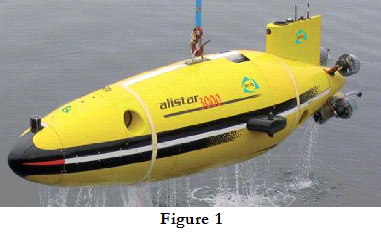
\includegraphics[width=.95\textwidth]{png/fig_01}
\end{center}
\end{minipage}

\vspace{.25cm}}

\section{Présentation du drone}
\ifthenelse{\boolean{prof}}{}{
Le sous-marin autonome d’inspection, objet de cette étude, est développé par la société ECA, localisée à Toulon (Var), spécialisée dans la robotique terrestre et sous-marine pour les environnements hostiles où l’homme ne peut pas intervenir directement (Vidéos disponibles sur \url{http://www.eca-robotics.com}).

L’ALISTAR 3000 (figure 1) est un engin sous-marin autonome qui entre dans la catégorie des « AUV » (Autonomus Underwater Vehicle) capable d’effectuer une grande variété de tâches d’inspection sur les champs pétrolifères Offshore jusqu’à une profondeur de 3 000 m. Une fois la mission d’inspection établie et programmée, il offre la possibilité de recueillir des données vidéo (caméra) et sonars (latéral et à balayage) des installations sous-marines visitées (pipeline, tête de puits, . . .). 
Le profil d’une mission type de ce sous-marin (figure 2) se décompose par l’enchainement temporel de cinq phases distinctes :
\begin{enumerate}
\item une phase de préparation du sous-marin et de mise à l’eau ;
\item une phase de descente afin de rejoindre le point de départ de son travail d’inspection ;
\item une phase d’inspection ;
\item une phase de remontée à la surface ;
\item une phase de récupération du sous-marin.
\end{enumerate}

\begin{center}
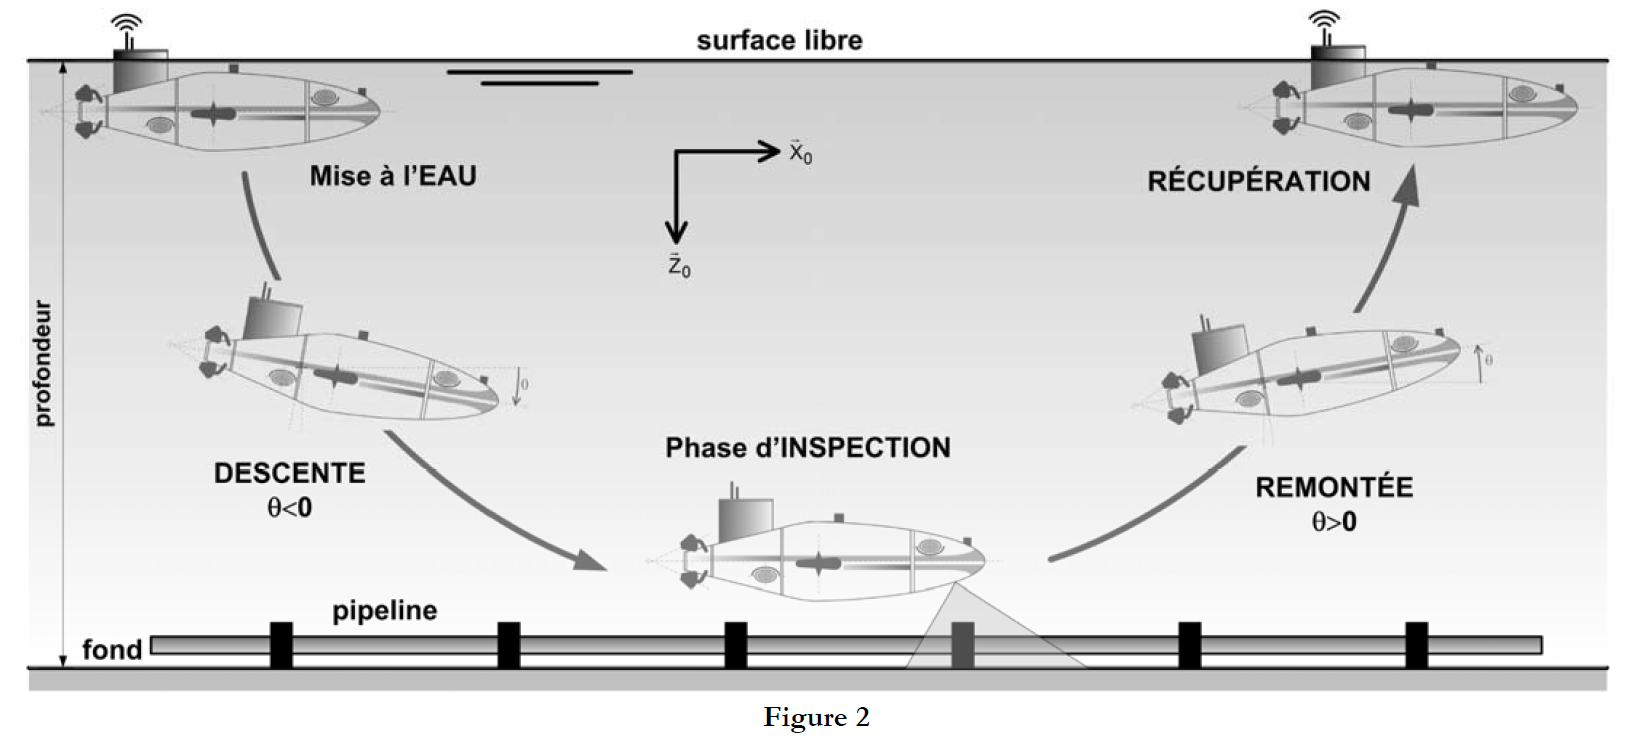
\includegraphics[width=.95\textwidth]{png/fig_02}
\end{center}
Pour se déplacer, l’ALISTAR est pourvu de 8 propulseurs : 4 propulseurs principaux arrière, 2 propulseurs latéraux avant et arrière et 2 propulseurs verticaux gauche et droite (architecture et localisation figure 3). Cette structure assure une excellente manœuvrabilité dans l’espace. Chaque propulseur est constitué d’un moteur électrique, d’un réducteur et d’une hélice.

\begin{center}
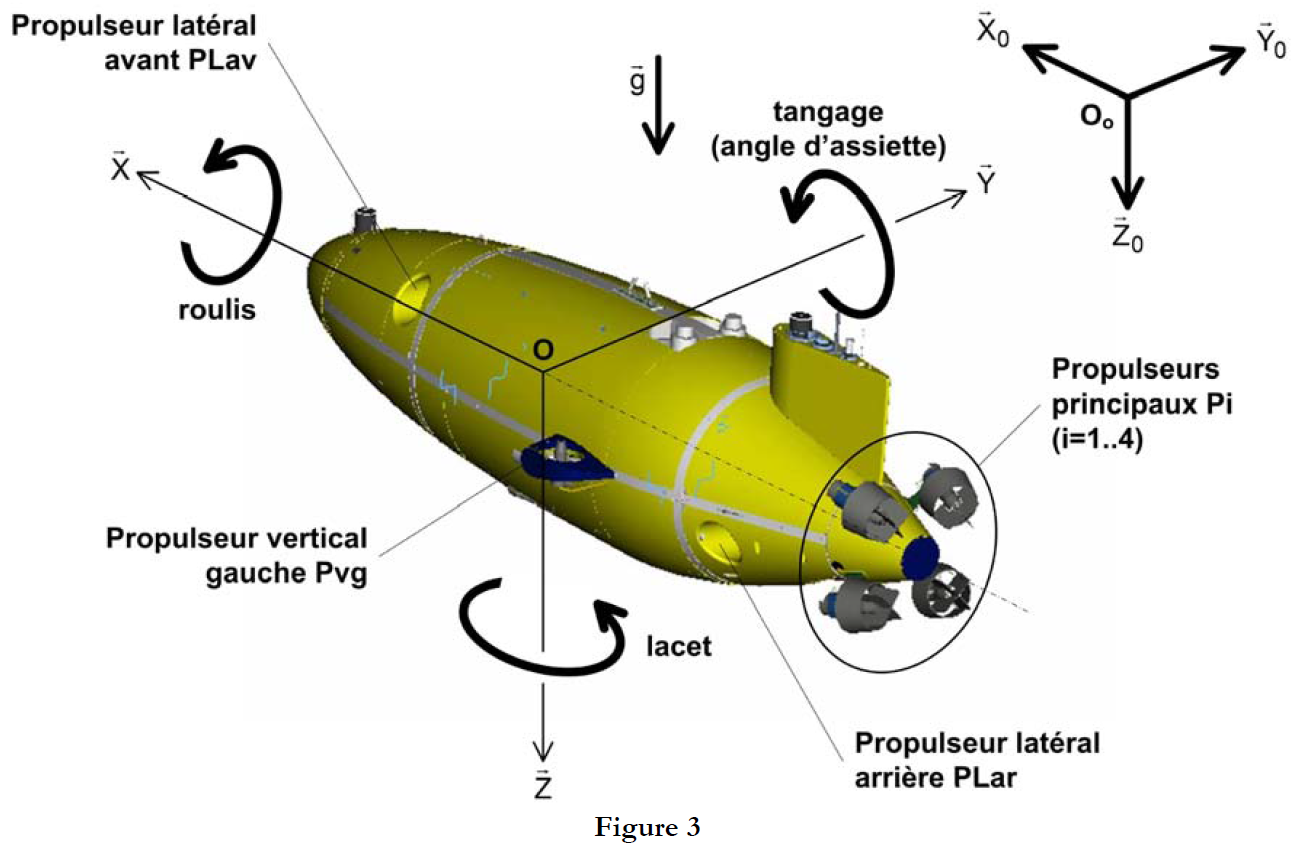
\includegraphics[width=.8\textwidth]{png/fig_03}
\end{center}


Comme le montre la figure 4, l’ALISTAR peut être commandé soit par un guidage automatique soit par une commande de type manuel (joystick). Dans le cas autonome, des consignes de pilotage préalablement définies sont fournies au système de commande. Différents capteurs (Doppler vitesse, gyro, compas, profondimètre altimètre, GPS) renseignent le système de commande sur le déplacement de l’ALISTAR. La caméra et le sonar permettent de recueillir les informations sur le pipeline, ces informations peuvent être stockées dans la mémoire du système de commande ou communiquées en temps réel à l’utilisateur via l’antenne.

\begin{center}
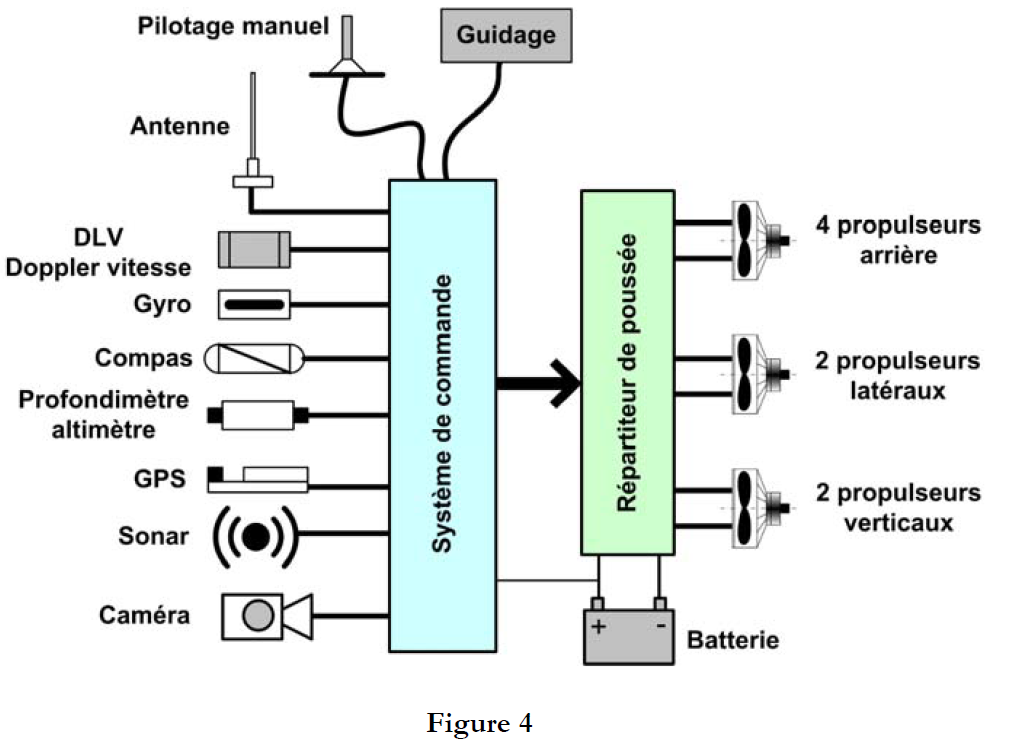
\includegraphics[width=.8\textwidth]{png/fig_04}
\end{center}

Le système de commande traite l’ensemble des informations pour élaborer les consignes de pilotage du répartiteur de poussée. Chaque moteur du propulseur est alors piloté individuellement pour diriger l’ALISTAR.

Dans la phase d’inspection d’un pipeline, l’ALISTAR enregistre une image de la structure externe du pipeline et effectue un balayage sonar. La qualité de ces enregistrements dépend fortement de la qualité du contrôle du déplacement de l’ALISTAR notamment en ce qui concerne la vitesse de déplacement de l’ALISTAR au dessus du pipeline. Différents essais ont montré que la vitesse optimale était de 2 nœuds soit $1,028\; m\cdot s^{-1}$.


La mission de l’ALISTAR est définie par les exigences ci-dessous. Nous nous limiterons ici aux exigences techniques :
\begin{itemize}
\item le drone doit pouvoir se déplacer dans le milieu marin;
\item le drone doit pouvoir détecter  le pipeline;
\item le drone doit pouvoir suivre le pipeline;
\item le drone doit pouvoir filmer et stocker les informations.
\end{itemize}

Pour ces deux dernières exigences, on précise qu'une exigence dérivée liée aux contraintes extérieures et au type de caméra utilisé est que la vitesse de déplacement optimale pour l'inspection est de deux nœuds, soit $1,028\;m/s$.

A noter que cette dernière exigence est définie par un lien « refine » : dans la norme sysml, il est indiqué que ce type de lien permettait l'ajout de valeurs numériques pour le raffinement. Ceci sera admis.
}
\section{Analyse système}
\subsection{Diagramme de contexte}
\ifthenelse{\boolean{prof}}{}{
On donne ci-dessous le diagramme de contexte de l’ALISTAR :
\begin{center}
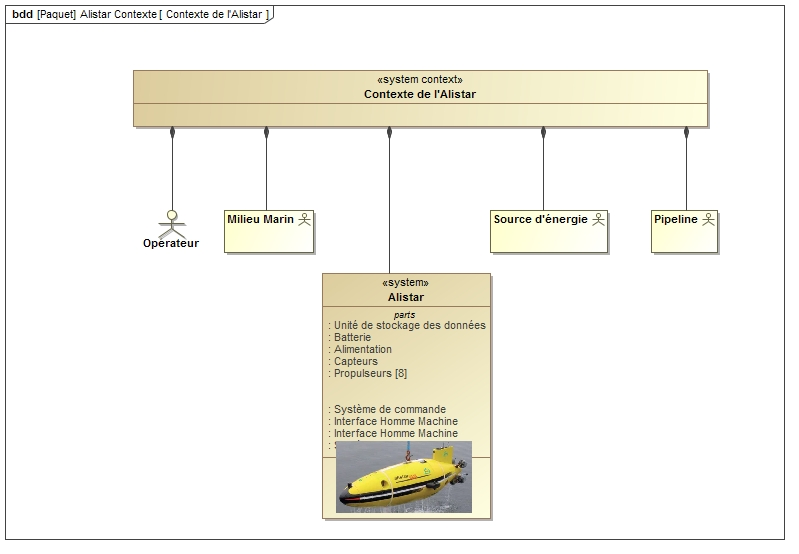
\includegraphics[width=.95\textwidth]{png/fig_05}
\end{center}
}

\subparagraph{}
\textit{Après avoir reproduit ce tableau sur votre copie, identifier les éléments du contexte présents dans chaque phase.}
\ifthenelse{\boolean{prof}}{
\begin{corrige}
\begin{center}
\begin{tabular}{|p{3cm}|p{3cm}|p{3cm}|p{3cm}|p{3cm}|}
\hline
 & Opérateur & Milieu Marin & Source d'énergie & Pipeline \\
\hline
Phase de présentation avant mise à l'eau &  \begin{center} X \end{center} & & \begin{center} X \end{center} & \\
\hline
Phase de descente & \begin{center} X si pilotage manuel\end{center} & \begin{center} X \end{center}& & \\
\hline
Phase d'inspection  & \begin{center} X si pilotage manuel\end{center} & \begin{center} X \end{center}& & \begin{center} X \end{center}\\
\hline
\end{tabular}
\end{center}
\end{corrige}}{
\begin{center}
\begin{tabular}{|p{3cm}|p{3cm}|p{3cm}|p{3cm}|p{3cm}|}
\hline
 & Opérateur & Milieu Marin & Source d'énergie & Pipeline \\
\hline
Phase de présentation avant mise à l'eau & & & & \\
\hline
Phase de descente & & & & \\
\hline
Phase d'inspection  & & & & \\
\hline
\end{tabular}
\end{center}
}


\subsection{Diagramme d'exigences}

On donne sur le document réponse DR 1 le diagramme d'exigence partiel de l’ALISTAR.

\subparagraph{}
\textit{Compléter celui-ci à partir des informations du sujet.}

\ifthenelse{\boolean{prof}}{
\begin{corrige}
\begin{center}
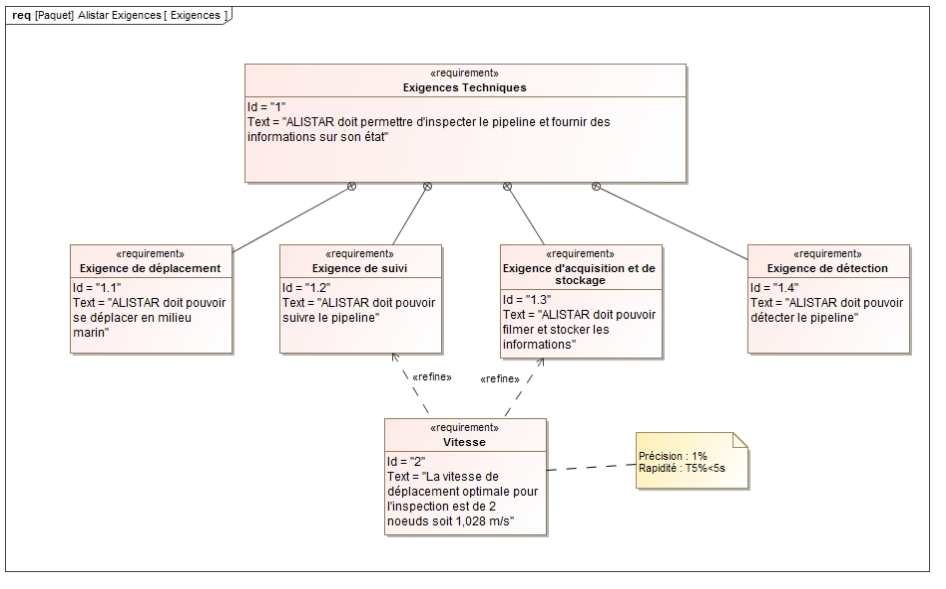
\includegraphics[width=.95\textwidth]{png/Q2}
\end{center}
\end{corrige}
}{}

\subsection{Diagramme des cas d'utilisation et cahier des charges associé}
\ifthenelse{\boolean{prof}}{}{
On donne ci dessous le diagramme des cas d'utilisation.

\begin{center}
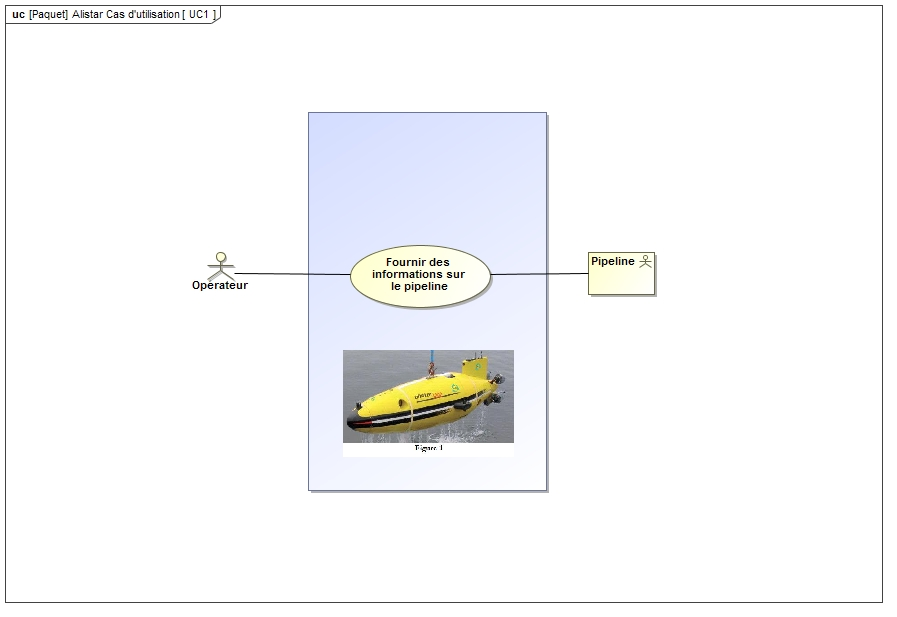
\includegraphics[width=.95\textwidth]{png/fig_06}
\end{center}
}

\subparagraph{}
\textit{Expliquer en une phrase ce que ce diagramme retranscrit comme information.}

\ifthenelse{\boolean{prof}}{
\begin{corrige}
L’utilisateur doit pouvoir acquérir des informations sur le pipeline en utilisant l’Alistar.
\end{corrige}
}{}

\ifthenelse{\boolean{prof}}{}{
Dans ce qui suit, nous nous limiterons à l'exigence liée au suivi du pipeline et à la maîtrise de ce suivi. Le critère lié à la vitesse de suivi sera défini par le cahier des charges partiel suivant :

\begin{center}
\begin{tabular}{|p{4cm}|p{4cm}|p{4cm}|p{4cm}|}
\hline
Exigence & Critère & Niveau & Flexibilité \\
\hline
\multirow{4}{4cm}{Le drone doit pouvoir suivre le pipeline.}
&
Vitesse de déplacement & $1,012 \;m/s$ & Non définie \\ \cline{2-4}
& Erreur en régime stationnaire pour une entrée en échelon de vitesse & 1\% & Non définie \\ \cline{2-4}
& Rapidité & $Tr 5\% < 5s$ & Non définie \\ \cline{2-4}
& Amortissement & Parfait, pas de dépassement & Non définie \\ \hline
\end{tabular}
\end{center}}

\subsection{Description structurelle du drone – Chaîne d'énergie et d'information}


On propose sur le document réponse DR2 un diagramme bdd du drone.

\subparagraph{}
\textit{Relier les blocs GPS, Caméra, Sonar, moteur et hélice à un des blocs déjà définis.}

\ifthenelse{\boolean{prof}}{
\begin{corrige}
\begin{center}
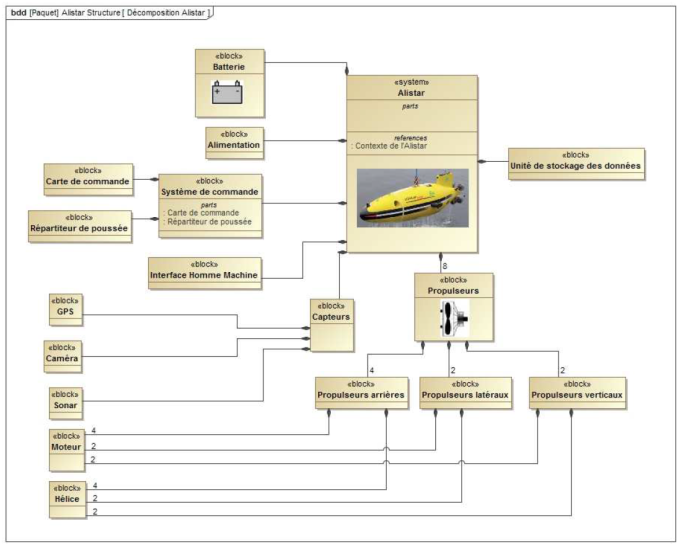
\includegraphics[width=.95\textwidth]{png/Q4.png}
\end{center}
\end{corrige}
}{}


On propose alors un diagramme ibd  (DR3).

\subparagraph{}
\textit{Compléter le diagramme en faisant apparaître pour chaque flux sa nature (Matière – Energie – Information).}

\ifthenelse{\boolean{prof}}{
\begin{corrige}
\begin{center}
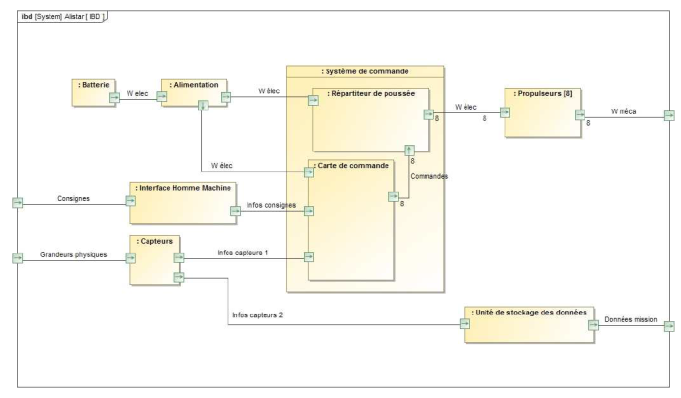
\includegraphics[width=.95\textwidth]{png/Q5.png}
\end{center}
\end{corrige}
}{}

\subparagraph{}
\textit{Faire apparaître en couleur la chaîne d'énergie sur le diagramme ibd.}

%\ifthenelse{\boolean{prof}}{
%\begin{corrige}
%\end{corrige}
%}{}

\subparagraph{}
\textit{En utilisant la question précédente compléter le diagramme chaîne d'énergie et d'information du document réponse DR 4.}

\ifthenelse{\boolean{prof}}{
%\begin{corrige}
%\begin{center}
%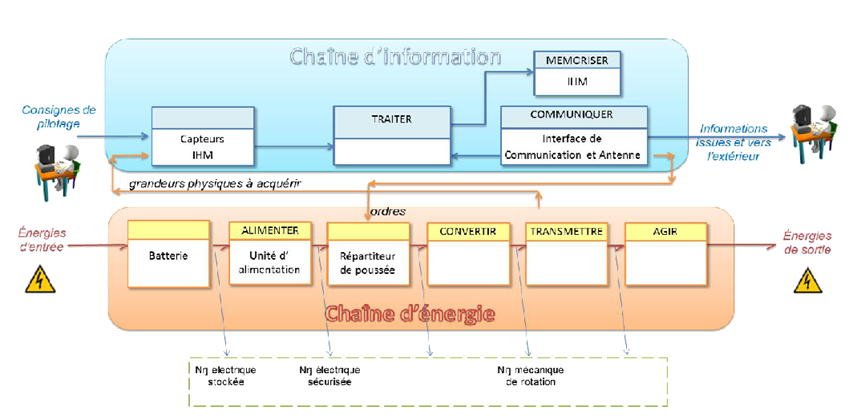
\includegraphics[width=.95\textwidth]{png/Q7.png}
%\end{center}

%\end{corrige}
}{}


\section{Modélisation du système}
\ifthenelse{\boolean{prof}}{}{
Faisant suite à la phase de descente sur zone d’inspection à la profondeur souhaitée et l’AUV étant supposé initialement immobile, la phase d’inspection proprement dite peut débuter.

Pour cela, l’AUV doit évoluer parallèlement au pipeline à inspecter que l’on suppose, dans un souci de simplification, rectiligne et posé horizontalement au fond de la mer.
On rappelle qu’afin d’acquérir correctement une image du pipeline, le déplacement de l’AUV doit s’effectuer à une vitesse constante et demeurer à une distance maîtrisée de ce dernier. Il est donc nécessaire de posséder une modélisation performante du comportement global de l’engin durant toute la phase d’inspection, condition indispensable à son contrôle.


\subsection{Modèle de connaissance du comportement du moteur à courant continu}

Un modèle simple et convenable pour ce type de moteur est:
\begin{eqnarray*}
U_m(t)=e(t)+Ri(t) \\
C_m(t)=K\cdot i(t) \\
e(t)=K\cdot n(t) \\
C_m(t) = J\dfrac{dn(t)}{dt}
\end{eqnarray*}

D’un point de vue mécanique, on suppose que l’axe est soumis à un couple moteur $C_m(t)$. On note $J$ l’inertie de l’axe du moteur. On note par ailleurs:
\begin{itemize}
\item $U_m(t)$ l'alimentation électrique du moteur (en Volt);
\item $i(t)$ l'intensité du courant (en Ampère);
\item $n(t)$ la vitesse de rotation du moteur (en rad/s);
\item $R$ la résitance de l'induit (en Ohm);
\item $e(t)$ la force contre électromotrice (en Volt);
\item $K$ la constante de couple / de force contre électro motrice.
\end{itemize}

On note classiquement $p$ la variable de Laplace et $U_m(p)$, $N(p)$ , $I(p)$, $E(p)$ et $C_m(p)$ les transformées de Laplace des variables précédentes.
}

\subparagraph{}
\textit{En précisant les hypothèses nécessaires, donner les transformées de Laplace des équations 1 à 4.}

\ifthenelse{\boolean{prof}}{
\begin{corrige}
Les conditions initiales étant nulles et les fonctions étant causales (fonctions nulles pour $t\leq 0$), on a donc : 
\begin{eqnarray*}
U_m(p)=E(p)+RI(p) \\
C_m(p)=K\cdot I(p) \\
E(p)=K\cdot N(p) \\
C_m(p) = JpN(p)
\end{eqnarray*}

\end{corrige}
}{}

\subparagraph{}
\textit{Par le calcul, définir la fonction de transfert du moteur notée $H(p)$ telle que $N(p)=H(p)\cdot U_m(p)$. Cette fonction de transfert s'exprimera uniquement en fonction de $R$, $K$ et $J$.}

\ifthenelse{\boolean{prof}}{
\begin{corrige}
On a  :
$$
N(p) = \dfrac{C_m(p)}{Jp} 
\Leftrightarrow 
N(p) = \dfrac{K}{Jp} \cdot I(p)
\Leftrightarrow 
N(p) = \dfrac{K}{RJp} \cdot \left(U_m(p)-E(p)\right)
\Leftrightarrow 
N(p) = \dfrac{K}{RJp} \cdot \left(U_m(p)-K\cdot N(p)\right)
$$
Au final, 
$$
H(p)=
\dfrac{N(p)}{U_m(p)}= \dfrac{\dfrac{K}{RJp} }{\dfrac{K^2}{RJp} +1}
=\dfrac{K}{K^2 +RJp}
=\dfrac{1/K}{1 +\dfrac{RJ}{K^2}p}
$$
\end{corrige}
}{}

\subparagraph{}
\textit{Mettre $H(p)$ sous forme canonique et déterminer ses paramètres caractéristiques.}

\ifthenelse{\boolean{prof}}{
\begin{corrige}
$H(p)$ peut se mettre sous la forme $H(p)=\dfrac{K_m}{1+\tau_m p}$ avec 
$K_m=\dfrac{1}{K}$ et $\tau_m=\dfrac{RJ}{K^2}$.

\end{corrige}
}{}


\section{Analyse et validation des performances.}
\ifthenelse{\boolean{prof}}{}{
On se place toujours durant la phase d’inspection d’un pipeline rectiligne et horizontal. La qualité des enregistrements dépend fortement de la qualité du contrôle du déplacement de l’AUV que ce soit en vitesse de déplacement ou en régulant la distance qui le sépare du pipeline. En ce qui concerne spécifiquement la vitesse de suivi, le schéma-bloc modélisant la commande asservie du sous-marin peut se mettre sous la forme suivante :

\begin{center}
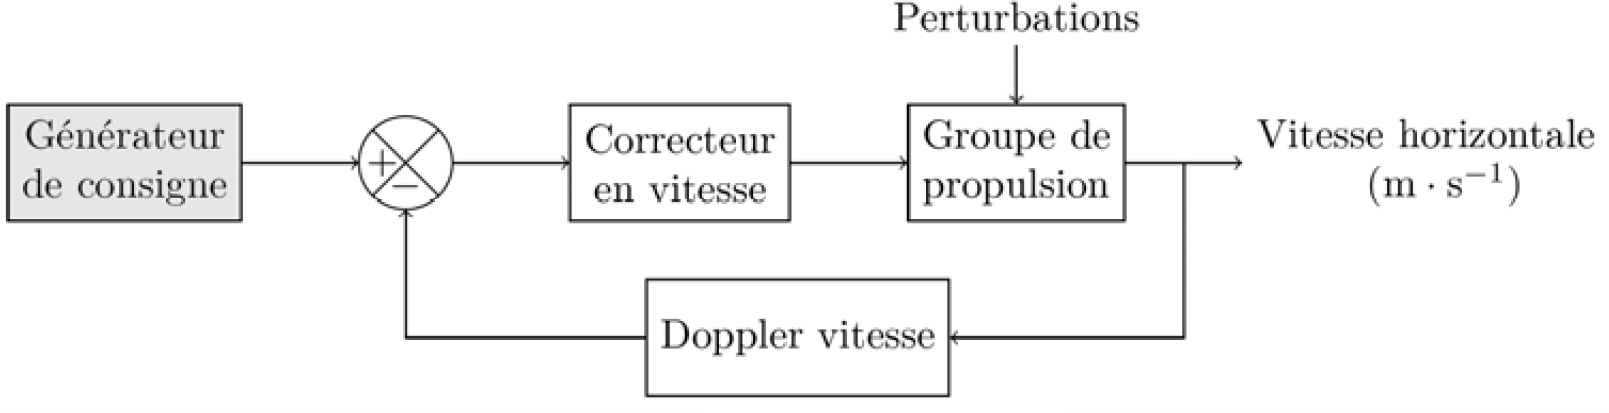
\includegraphics[width=.95\textwidth]{png/fig_07}
\end{center}

Une étude expérimentale de l’AUV permet d'obtenir la courbe de réponse donnée sur le document réponse DR 4 pour le groupe de propulsion. On peut alors procéder à une identification du bloc noté $H_2(p)$ ci-dessous :

\begin{center}
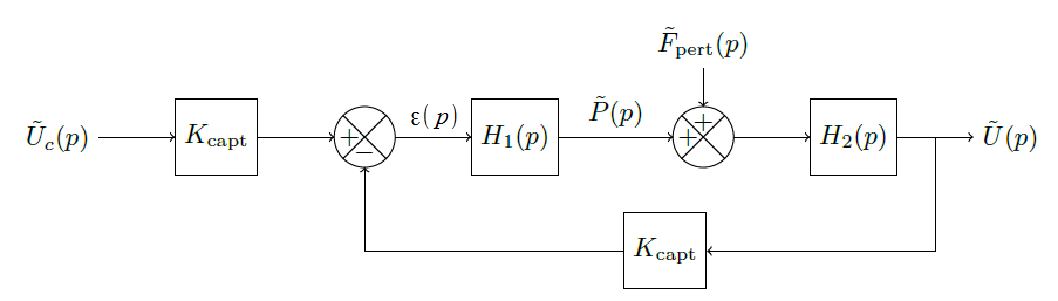
\includegraphics[width=.95\textwidth]{png/fig_08}
\end{center}

Pour ne pas confondre avec le schéma bloc global non linéaire (non donné ici), toutes les variables linéarisées seront notées avec un « tilde ». On a donc :
\begin{itemize}
\item $\tilde{u}_c(t)$ représente la consigne en vitesse (en m/s);
\item $\tilde{u}(t)$ la vitesse de déplacement de l’AUV (en m/s);
\item $\tilde{p}(t)$ la poussée totale (en N);
\item $\tilde{f}_{pert}(t)$ l’effort de perturbation (en N) lié aux conditions changeantes de fonctionnement.
\end{itemize}

On note classiquement $p$ la variable de Laplace et $\tilde{U_c}(p)$, $\tilde{U}(p)$ , $\tilde{P}(p)$ et $\tilde{F}_{pert}(p)$ les transformées de Laplace des variables précédentes.

On impose que $H_1(p)=G\cdot C(p)$ avec $G=94 N/V$ et $C(p)$ représentant la fonction de transfert du correcteur. 

Par souci de simplification, on impose $K_{capt}=1V/m$. $H_2$ a été déterminée expérimentalement : $\tilde{H_2}(p)=\dfrac{\tilde{K}}{1+\tilde{\tau}p}$ avec $\tilde{K}=5\cdot 10^{-3}\; USI$ et $\tilde{\tau} = 12\; s.$
}
\subsection{Étude des performances de précision de l'asservissement non corrigé}

On suppose que le correcteur est unitaire, soit $C(p)=1$. Par ailleurs, on supposera ici les perturbations nulles.

\subparagraph{}
\textit{Calculer la FTBO puis $\varepsilon(p)$. }

\ifthenelse{\boolean{prof}}{
\begin{corrige}
Dans un premier temps, 
$$FTBO(p)=H_1(p)\cdot H_2(p) \cdot K_{capt} = 
K_{capt} G \cdot \dfrac{\tilde{K}}{1+\tilde{\tau}p}$$

$\varepsilon(p)$ peut être directement déterminé ainsi : 
$$
\varepsilon(p)= \dfrac{1}{1+FTBO(p)} \cdot K_{capt} \tilde{U}_c(p) 
=\dfrac{K_{capt}}{1+ K_{capt} G \cdot \dfrac{\tilde{K}}{1+\tilde{\tau}p}} \tilde{U}_c(p) 
=K_{capt}\dfrac{1+\tilde{\tau}p}{1+\tilde{\tau}p+ K_{capt} G  \tilde{K}}  \tilde{U}_c(p) 
$$
En mettant cette expression sous forme canonique, on obtient :
$$
\varepsilon(p)
=\dfrac{K_{capt}}{1+\tilde{K}GK_{capt}} \cdot \dfrac{1+\tilde{\tau}p}{1+\dfrac{\tilde{\tau}}{1+\tilde{K}GK_{capt}}p}  \tilde{U}_c(p) 
$$
\end{corrige}
}{}

\subparagraph{}
\textit{On considère une position de consigne variant en échelon d'amplitude $U_{c0}$ . Donner l'expression de la transformée de Laplace $\tilde{U_c}(p)$ de ce signal d'entrée.}

\ifthenelse{\boolean{prof}}{
\begin{corrige}
Une entrée échelon se modélise ainsi : 
$$
\tilde{U_c}(p) = \dfrac{U_{c0}}{p}
$$
\end{corrige}
}{}

\subparagraph{}
\textit{\`A partir du théorème de la valeur finale, calculer la valeur de l'erreur en régime permanent pour une entrée en échelon en fonction de $G$ et $\tilde{K}$.}

\ifthenelse{\boolean{prof}}{
\begin{corrige}
On a : 
$$
e_{rs}=
\lim\limits_{t\to \infty} \varepsilon(t) 
= \lim\limits_{p\to 0} p\varepsilon(p) 
= \lim\limits_{p\to 0} p \cdot \dfrac{U_{c0}}{p} \cdot \dfrac{K_{capt}}{1+\tilde{K}GK_{capt}} \cdot \dfrac{1+\tilde{\tau}p}{1+\dfrac{\tilde{\tau}}{1+\tilde{K}GK_{capt}}p} 
= \dfrac{K_{capt}U_{c0}}{1+\tilde{K}GK_{capt}}
$$
\end{corrige}
}{}

Indépendamment du résultat trouvé précédemment, on prendra :
$$
e_{rs}=\dfrac{K_{capt}}{1+G\tilde{K}K_{capt}}\cdot U_{c0}
$$

\subparagraph{}
\textit{Le système est-il précis vis-à-vis de cette entrée en échelon? Calculer la valeur numérique de l'erreur en régime permanent pour une entrée en échelon relative (en pour-cents).}

\ifthenelse{\boolean{prof}}{
\begin{corrige}
$$
e_{rs}=\dfrac{1}{1+94\cdot 5\cdot 10^{-3}\cdot 1}\cdot U_{c0}
=0,68 \cdot U_{c0}
$$
\end{corrige}
}{}



\subparagraph{}
\textit{\`A partir de la réponse à la question précédente, conclure quant au respect du cahier des charges.}

\ifthenelse{\boolean{prof}}{
\begin{corrige}
Le cahier des charges indique une erreur statique admissible de 1\% ce qui est largement inférieur aux 68\% calculés. Le système tel qu'il est modélisé actuellement ne respecte donc pas le cahier des charges. 
\end{corrige}
}{}



\subsection{Étude des performances de précision de l'asservissement corrigé}
\ifthenelse{\boolean{prof}}{}{
On cherche à présent la valeur du gain de correction $C(p) = K_{cor}$ permettant de vérifier toutes les performances du cahier des charges fonctionnel. Par ailleurs, on supposera toujours les perturbations nulles.

Une étude non demandée ici, se basant sur l'analyse de précision faite précédemment, permettrait de définir le gain $K_{cor} = 211$ pour assurer la précision du cahier des charges.

Pour définir les deux autres performances du CdCf, on définit la fonction de transfert en boucle fermée notée: $FTBF(p)$ telle que $\tilde{U}(p)=FTBF(p)\cdot \tilde{U}_C(p)$.
}

\subparagraph{}
\textit{Calculer $FTBF(p)$ et donner son expression en fonction des paramètres caractéristiques du modèle. Quel est l'ordre de cette fonction de transfert?}
\ifthenelse{\boolean{prof}}{
\begin{corrige}
La fonction de transfert en boucle fermée peut se calculer ainsi :
$$
FTBF(p)=\dfrac{K_{capt}H_1(p)H_2(p)}{1+K_{capt}H_1(p)H_2(p)}
=\dfrac{K_{capt}\cdot G \cdot K_{cor}\cdot\dfrac{\tilde{K}}{1+\tilde{\tau}p}}{1+K_{capt}\cdot G \cdot K_{cor}\cdot \dfrac{\tilde{K}}{1+\tilde{\tau}p}}
=\dfrac{K_{capt}\cdot G \cdot K_{cor}\cdot \tilde{K}}{1+\tilde{\tau}p+K_{capt}\cdot G \cdot K_{cor}\cdot \tilde{K}}
$$
Ce système est du premier ordre. Mettons le sous forme canonique :
$$
FTBF(p)
=\dfrac{\dfrac{K_{capt}\cdot G \cdot K_{cor}\cdot \tilde{K}}{1+K_{capt}\cdot G \cdot K_{cor}\cdot \tilde{K}}}{1+\dfrac{\tilde{\tau}}{1+K_{capt}\cdot G \cdot K_{cor}\cdot \tilde{K}}p}
$$
\end{corrige}
}{}

\subparagraph{}
\textit{Donner sans calculs l'expression analytique puis la valeur du temps de réponse à 5\%. Conclure vis-à-vis du cahier des charges fonctionnel.}

\ifthenelse{\boolean{prof}}{
\begin{corrige}
Le système étant du premier ordre, le temps de réponse à 5\% est le triple du temps de réponse. On a donc, 
$$
tr_{5\%}=3\cdot \dfrac{\tilde{\tau}}{1+K_{capt}\cdot G \cdot K_{cor}\cdot \tilde{K}}
= 3\cdot \dfrac{12}{1+1\cdot 94 \cdot 211 \cdot 5\cdot 10^{-3}} = 0,36\; s.
$$

Le temps de réponse à 5\% est inférieur aux 5 secondes imposées par le cahier des charges. Ce dernier est donc vérifié. 

\end{corrige}
}{}

\subparagraph{}
\textit{\`A partir de l'expression de la $FTBF(p)$, conclure quant au critère d'amortissement.}

\ifthenelse{\boolean{prof}}{
\begin{corrige}
Le système étant du premier ordre, il n'y a donc pas de dépassement. Le cahier des charges est donc vérifié. 
\end{corrige}
}{}

\section{Flottabilité et mouvement de plongée du drone Alistar}

\subsection{Étude générale de la flottabilité}
\ifthenelse{\boolean{prof}}{}{
L'objectif ici est de déterminer, en fonction des conditions de plongée, la valeur du lest à ajouter au sous-marin afin d’obtenir une flottabilité nulle à $3\, 000\; m$.

Afin de maîtriser le comportement d’un véhicule sous-marin en phase de plongée, on doit être capable de faire varier sa flottabilité. La flottabilité d’un corps en immersion représente la différence entre la poussée d’Archimède et l’action de pesanteur. La flottabilité (notée $\Phi$) dépend donc de la masse du corps (notée $m$), de son volume (noté $V$) et de la masse volumique de l’eau (notée $\rho$). On définit donc : $\Phi = \rho V - m$.

On rappelle que lors de la phase de pesée et de mise à l’eau, on doit avoir :
\begin{itemize}
\item une flottabilité nulle à $3\, 000\; m$ de profondeur ;
\item une flottabilité de $10\; kg$ en surface de manière à ce que les antennes et le système de communication demeurent émergés.
\end{itemize}

L’ALISTAR a été conçu afin de posséder une flottabilité nulle en surface en eau douce. Ses caractéristiques sont donc (dans l’air) : un volume $V_0 = 1,9772\;m^3$ et une masse $m = 1977,2 \; kg$. 

Lors d’une plongé à $3\, 000\; m$, sous l’effet de la pression, la masse volumique de l’eau de mer varie comme le montre la figure ci dessous (courbe de gauche). On remarque que la graduation de l’axe « profondeur » est croissante vers le bas.

Dans les mêmes conditions, sous l’effet de la pression de l’eau, le volume de l’AUV se modifie également comme le montre la figure ci dessous (courbe de droite). 

\textit{Remarque : par la suite, on supposera que les lois d'évolution des grandeurs de cette figure sont linéaires pour une profondeur supérieure à $50\;m$.}

\begin{center}
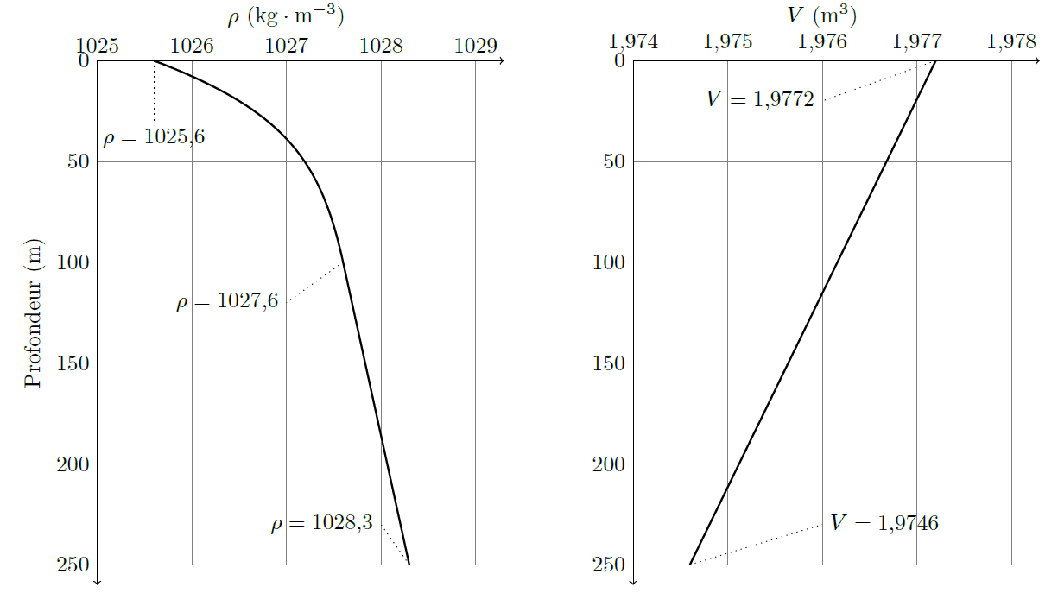
\includegraphics[width=.95\textwidth]{png/fig_09}
\end{center}


En effet, le sous-marin est constitué de deux parties : un squelette tubulaire supposé indéformable (cf. figure 5) dont la fonction est de supporter les différents éléments et sous-ensembles constituants l’AUV et une carène compressible formée en mousse haute densité qui sert à compléter le volume et à donner au sous-marin un profil hydrodynamique

\begin{center}
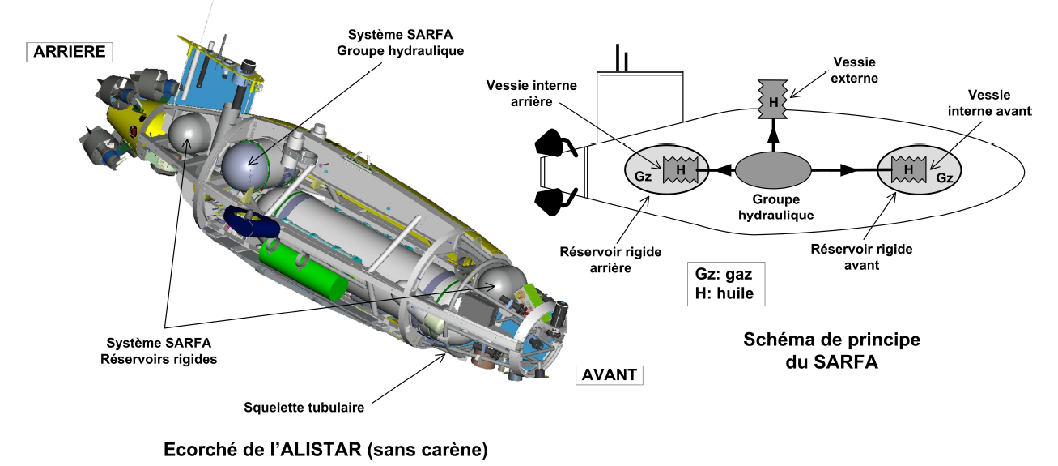
\includegraphics[width=.95\textwidth]{png/fig_10}

\textit{Figure 5}
\end{center}

}
\subparagraph{}
\textit{En supposant l'évolution linéaire de la variation de volume avec la profondeur, et en notant $l$, en $m$, cette profondeur, montrer que $V(l)=-0,0104\cdot l + 1977$, $V(l)$ étant en $dm^3$. Déterminer alors la réduction de volume en $dm^3$ de l’AUV à $3\,000\;m$ de profondeur. }

\ifthenelse{\boolean{prof}}{
\begin{corrige}
On a $V(3000)=1946 \;dm^3$. La réduction de volume est donc de $31,2\;dm^3$.
\end{corrige}
}{}

Une étude identique permettrait de définir la masse volumique à $3\,000\;m$ : $\rho(3000)=1\, 041,13 \; kg\cdot m^3$.


\subparagraph{}
\textit{Déterminer la masse du lest (en kg) à rajouter au sous-marin afin d’obtenir une flottabilité nulle à $3\,000\;m$.}

\ifthenelse{\boolean{prof}}{
\begin{corrige}
Pour obtenir une flottabilité nulle à 3000 m, il faut $\Phi=0$ soit $\rho(3000)\cdot V(3000)-m-l_{lest}=0$. On en déduit que  $m_{lest}=1041,13\cdot 1946\cdot10^{-3}-1977,2 = 48,84 \; kg$.
 

\end{corrige}
}{}

En utilisant la valeur du lest déterminée précédemment, on peut montrer que la flottabilité en surface n'est que de $1,77\;kg$. Cette valeur étant bien en dessous des $10\;kg$ exigés, il faut trouver une autre solution pour ce problème de flottabilité.

\subparagraph{}
\textit{Sachant que, lors de la mission, l’AUV ne prend ou ne rejette rien, sur quel paramètre structurel de l’AUV peut-on agir afin d’obtenir la flottabilité désirée ?}

\ifthenelse{\boolean{prof}}{
\begin{corrige}
Comme l'engin est considéré comme un milieu fermé (pas d'échange de matière), le seul paramètre sur lequel agir est le volume en gonflant ou dégonflant un élément.
\end{corrige}
}{}


\subsection{Système SARFA et mouvement de plongée}
\ifthenelse{\boolean{prof}}{}
{
Les phases de descente et de remontée ne sont pas des phases « utiles » ; elles sont transitoires. Le sous-marin doit donc les effectuer le plus rapidement possible en consommant le minimum d’énergie afin de conserver une autonomie suffisante pour la phase d’inspection. Le développement d’un Système Actif de Réglage de la Flottabilité et de l’Assiette (SARFA) entre dans cette perspective. Son objectif est de réduire (voire idéalement de supprimer) l’utilisation des différents propulseurs lors de ces phases transitoires.

Le SARFA (figure 5) se compose d’un groupe hydraulique (moteur électrique entraînant une pompe hydraulique assurant la circulation en circuit fermé et sous pression d’un fluide incompressible), de deux réservoirs rigides placés dans le plan médian (un vers l’avant et un vers l’arrière de l’AUV) remplis d’un gaz et dans lesquels on place une vessie de volume variable et enfin d’une vessie externe à l’AUV.

Comme le montre la figure 5, le fluide sous pression peut circuler dans les 3 vessies via un module de distribution (non représenté). Ainsi conçu, ce système permet de réaliser les deux fonctions du SARFA :
\begin{itemize}
\item le réglage de la flottabilité ; ce réglage s’effectue grâce à la variation du volume global du sous-marin. Le transfert du fluide hydraulique sous pression vers la vessie externe permet de gonfler cette dernière, affectant le volume de l’AUV et entraînant par voie de conséquence une modification de la poussée d’Archimède appliquée à l’engin ;
\item le réglage de l’angle d’assiette $\theta(t)$ (encore nommé angle de tangage) ; ce réglage s’effectue en déséquilibrant les masses de fluide hydraulique placées à l’intérieur des deux vessies avant et arrière. En transférant le fluide d’une vessie vers l’autre, il devient possible de modifier l’angle d’assiette indépendamment du réglage de la flottabilité. Schématiquement, par cette opération, on déplace le centre de gravité $G$ de l’engin.
\end{itemize}


\begin{center}
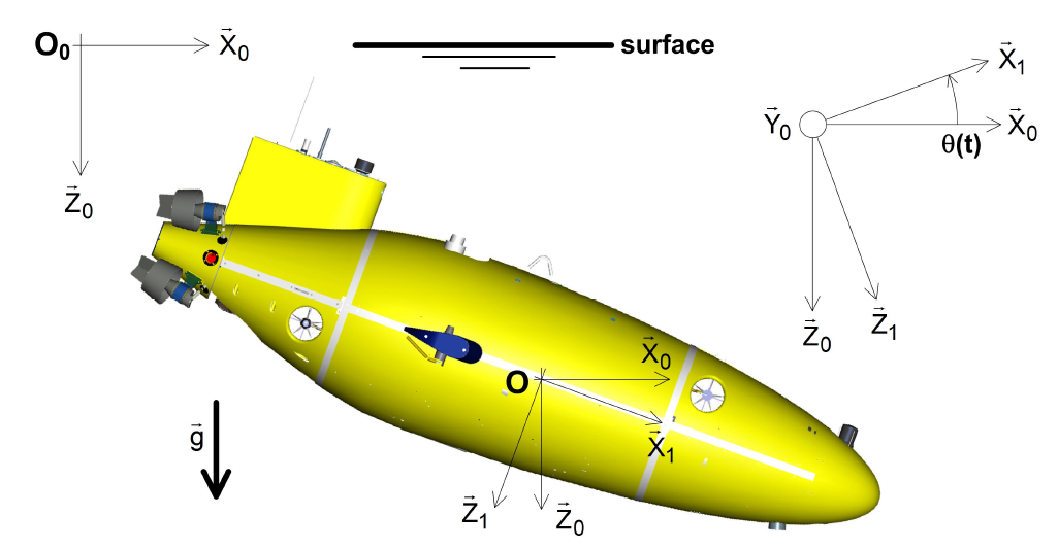
\includegraphics[width=.95\textwidth]{png/fig_11}
\end{center}

On suppose que le critère de flottabilité est vérifié.
}

\subparagraph{}
\textit{Expliquer le fonctionnement du SARFA pour permettre une plongée sans utiliser les propulseurs.}

\ifthenelse{\boolean{prof}}{
\begin{corrige}
Pour plonger il faut diminuer la flottabilité en dégonflant la vessie vers l'intérieur. En partant de la position initiale, le mouvement de plongée peut s'amorcer en dégonflant la vessie externe et en transférant du fluide de l'arrière vers l'avant pour déplacer le centre de gravité de l'AUV et lui donner un angle d'assiette négatif.
\end{corrige}
}{}
\ifthenelse{\boolean{prof}}{}{
\newpage

%\textbf{\texsf{Question 2}}
\begin{center}
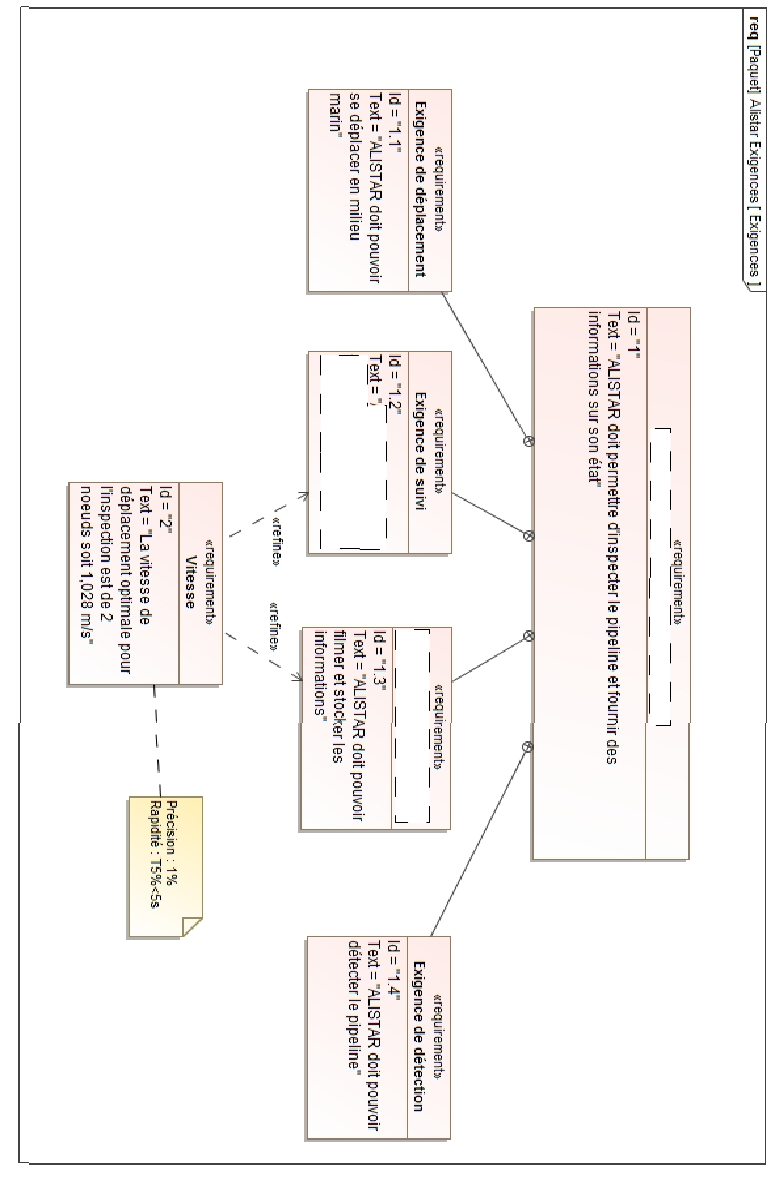
\includegraphics[height=\textheight]{png/fig_12}
\end{center}

\begin{center}
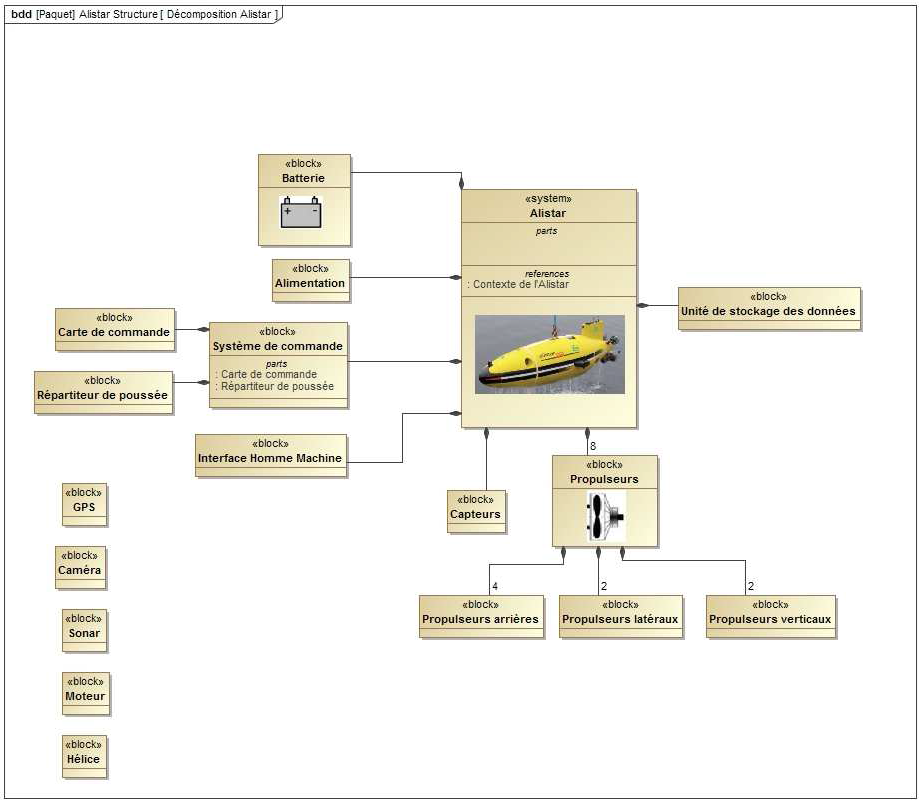
\includegraphics[width=.95\textwidth]{png/fig_13}
\end{center}

\begin{center}
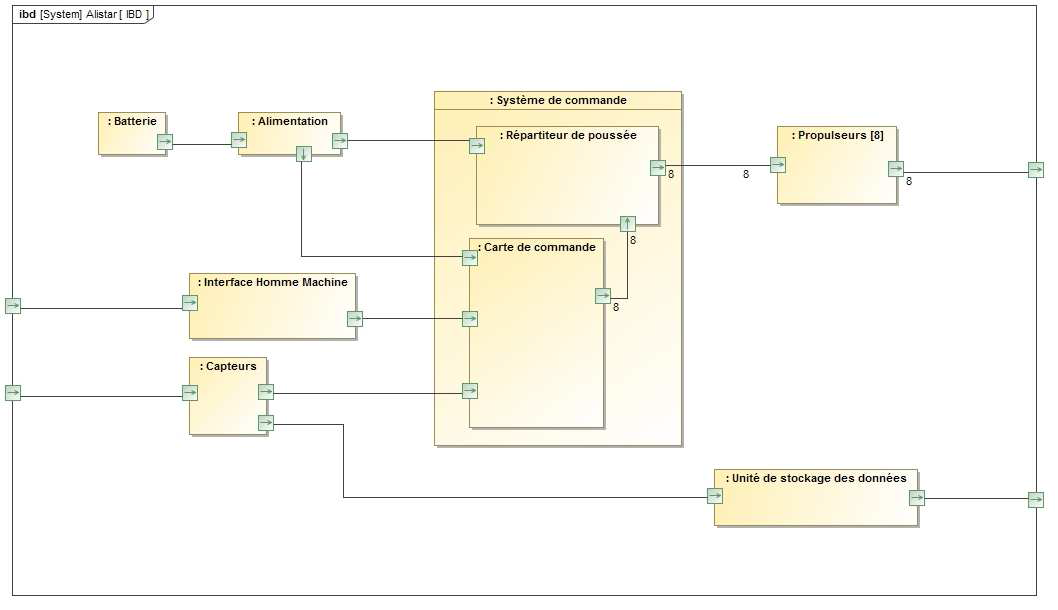
\includegraphics[width=.95\textwidth]{png/fig_14}
\end{center}

\begin{center}
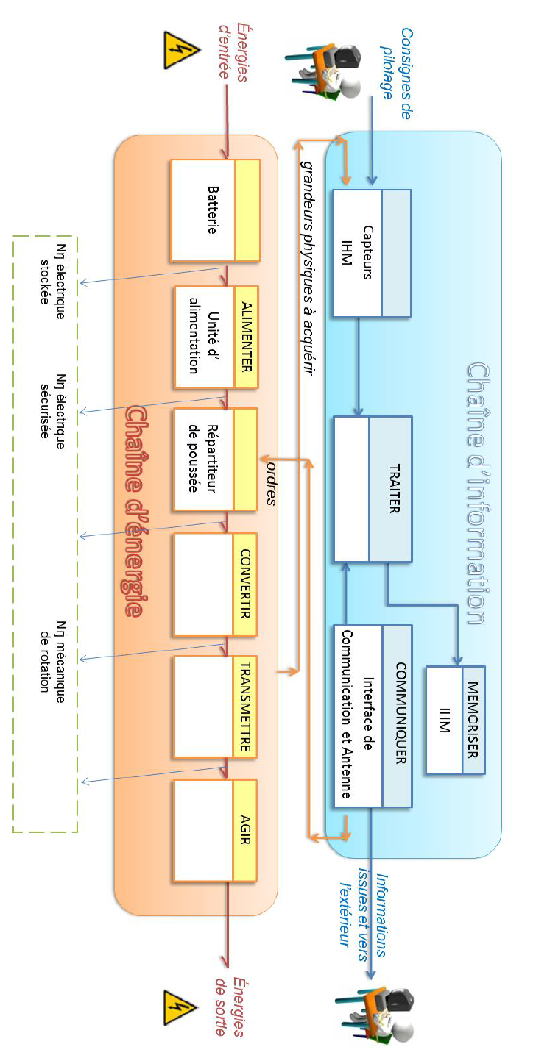
\includegraphics[height=\textheight]{png/fig_15}
\end{center}
}
\end{document}
